\newcommand{\definice}{\paragraph{Definice.}}

\chapter{Compilation and optimization}

In this chapter, we will discuss the composition of modern
programs, organization and size of their code-base. We proceed with an
overview of compilation stages, introduce optimization passses and link-time
optimization framework.

\section{Code-base organization and size}

Let us start by examining some of the code-bases for programs we use every day.
Many developers run Linux, Firefox (or other browser) and GCC, but
unless they are developing one of them, they do not really have a good idea of how large
they are. The chart in Figure \ref{figure-loc} shows historical development of
code-base size over the past 10 years for selected projects.

\begin{figure}[h!]
\centering
	\hspace{-1cm}\includegraphics{graphs/loc/loc.pdf}
\caption{Codebase size of Firefox, Chrome and GCC over time. \TODO{citace
	openhub.net}}
\label{figure-loc}
\end{figure}

It might be tempting to say that the code will be split into many libraries. It
however common practice to bundle many libraries into a single large binary. They
could be compiled into separate dynamic libraries, and linked at runtime. Figure
\ref{figure-firefox-objsize} shows 8 largest libraries contained in a standard
Firefox distribution. The size of main library is 66.39 MB, while the second
largest is only 1.51 MB. This is due to performance optimizations, as the developers
noticed a significant start-up cost of dynamic linking, and
bundled them together into a single library. This also means that compiler
link-time optimizing this library has to deal with enormous code base at once.

\begin{figure}[h!]
\centering
\includegraphics[angle=-90,trim=0 30 10 0,clip]{graphs/firefox-objsize/objsize.pdf}
\caption{Firefox 50.0.2 object sizes by binary}
\label{figure-firefox-objsize}
\end{figure}

We should keep these numbers in mind while designing a compiler. Compiler has
to keep up with the enormous code-base growth of projects, adding around 2
millions of lines of code each year.

\section{Program compilation}

Only the simplest programs consist of a single source file. Many programs have
tens, hundreds or even thousands of source files. This not only serves an
organizational purpose, but also allows the programmer to choose different
optimization flags for different files, or even write different parts in
different languages. A mechanism called {\sl separate compilation} is used to
compile and combine (link) all of them together, to form a finished program.
Figure \ref{figure-non-lto-workflow} shows the transformation using standard GCC
and Binutils (compiler and linker).

In this traditional model, first step is to compile every  source file into
object file. In this phase, a compiler is invoked and does all the work
necessary to convert source code into binary, including code generation. The
result is stored in an object file, including required metadata, for example,
symbol table. This step is independent for each source file, so they can be
processed in parallel. 

Second step consists of linking. The linker inspects all generated objects,
resolves required and provided symbols, dynamic libraris, and produces a
final executable. The linker usually does only minimal modifications to the code
in object files, as it only understands symbols and sections.

\begin{figure}[h!]
\centering
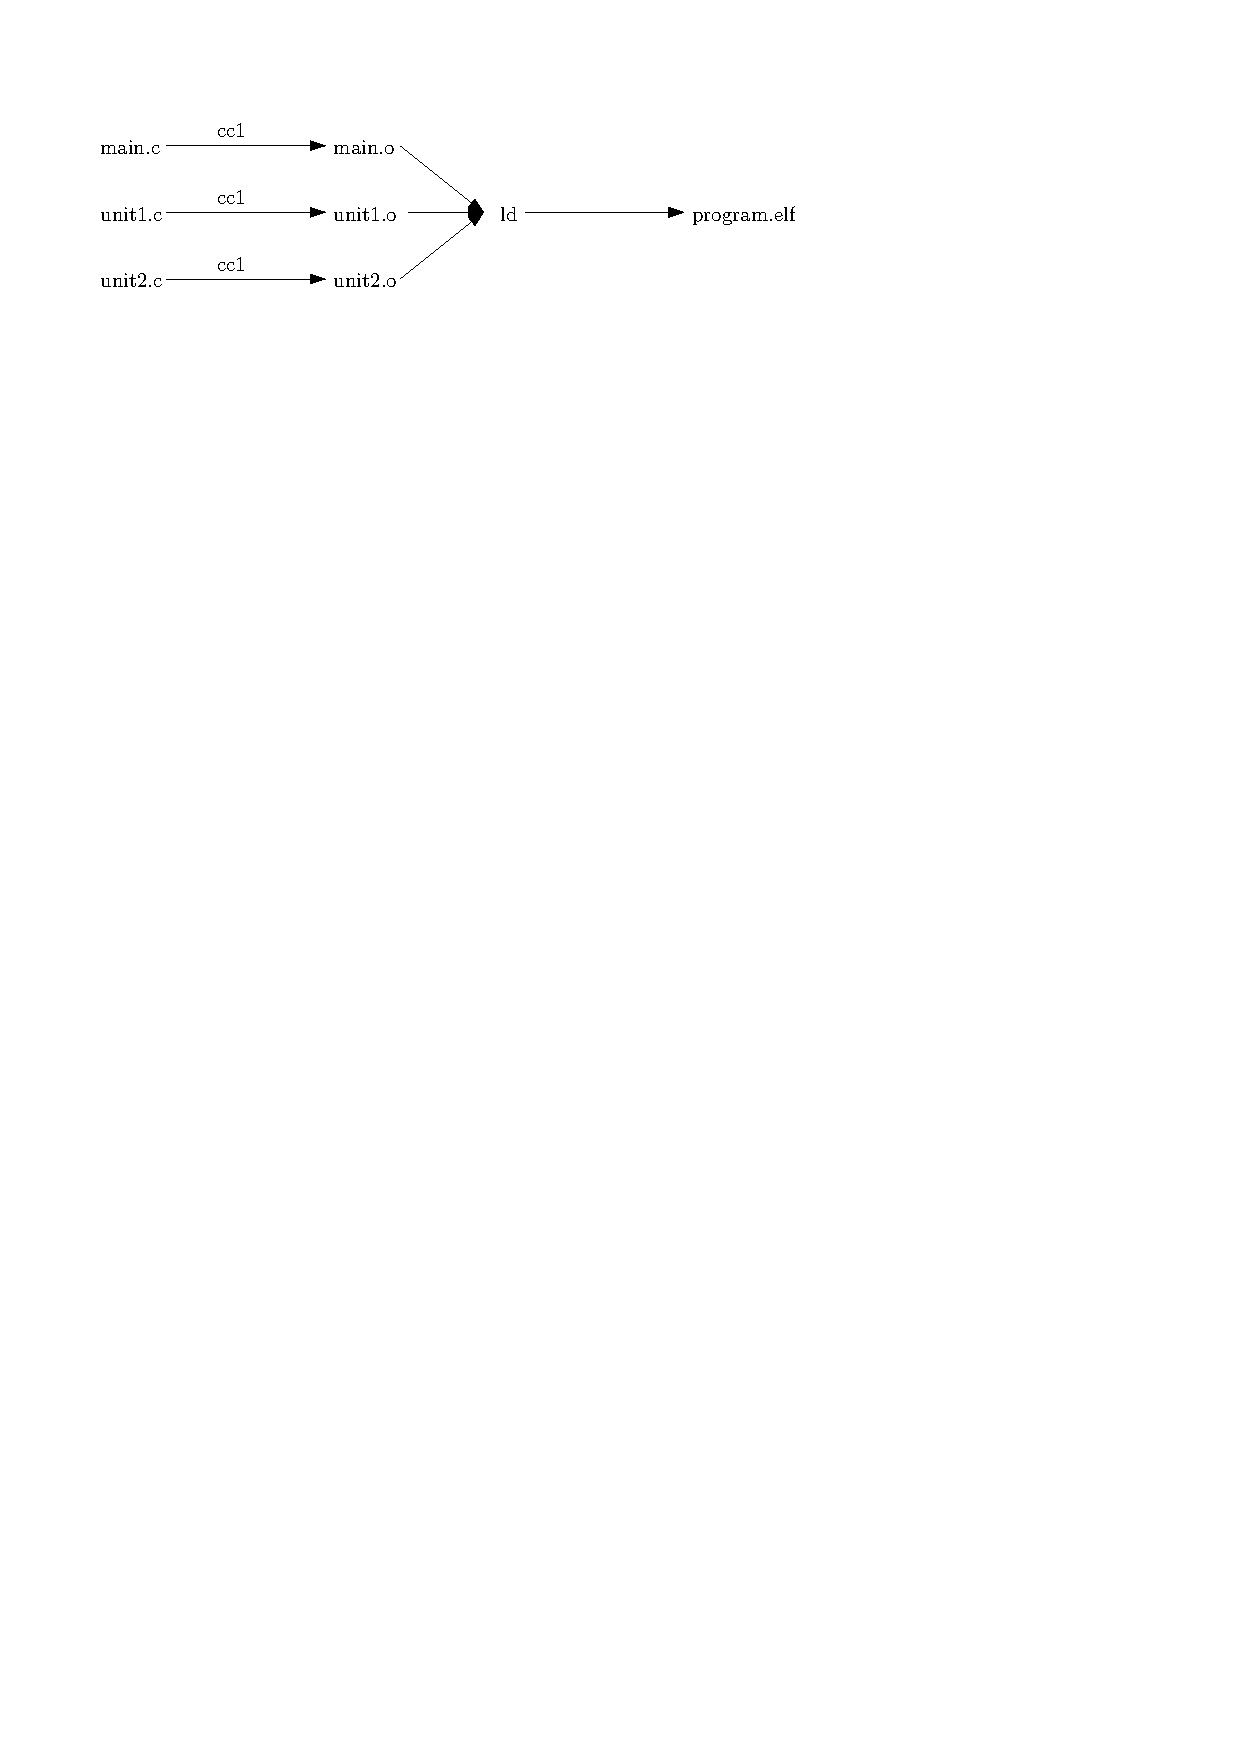
\includegraphics{./img/non-lto-workflow.pdf}
\caption{Standard workflow for separate compilation}
\label{figure-non-lto-workflow}
\end{figure}


\section{Compilation phases}

To compile a program written in a high-level programming language into a machine
code requires many steps. To make orientation easy, and to support code
re-usability, a compiler usually consists of the following high-level components:

\paragraph{Front End} parses the input language, builts abstract syntax
tree and converts it into an intermediate language (IL) which is used by the
middle-end.

\paragraph{Middle End} analyses the program represented in IL and performs most
highlevel optimizations. This includes splitting the code into basic blocks,
building a callgraph and control flow graph. Various optimizations are then
performed.

\paragraph{Back End} converts IL code into machine code, optimizing on the
lowest level. For example, it is able to schedule individual instructions and
allocate registers.

\bigskip

During this process multiple intermediary languages are used, sometimes more at
the same time (usually during transition to the lower-level language). For
example, GCC uses the following languages:

\begin{description}
	\item[GENERIC] is the highest-level IL used by the Front End, able to
		represent syntax trees and language-specific features.
	\item[GIMPLE] is tuple-based IL language, able to represent only simple
		expressions common to all languages. It is unable to represent many
		high-level constructs, for example, loops.
	\item[RTL] (Register Transfer Language) is a low level language similar to
		machine code, containing algebraicly described instructions, as should
		be generated.
\end{description}


\section{Link-time optimization}

Restricting the scope of optimization to a single compilation unit is an
important limitation to the optimizer. One example is devirtualization in C++,
which needs to build complete type inheritance graph to decide which virtual
function should be used. Literature usually assumes the compiler sees the whole
source, but as the class its descendants are usually in a separate
file, the compiler has no way of knowing that there is only one possible virtual
method, and devirtualize it.  This often happens when using Mock
objects\footnote{Objects that mimic some behavior, for example a piece of
hardware.} for testing.

The idea of interprocedural and link-time optimization (LTO) is old. 
It was already discussed in literature in 1970s \cite{Allen:1974,Allen:1976}.
One of the first industrial strength implementation of LTO optimizing compiler
was MIPSPro, which open-sourced in 2000 as Open64 under GNU GPL. The
compiler suite LLVM supports link-time optimization by design, from its first
release in 2002 \cite{lattner2002llvm}.  GCC was entering the link-time
optimization game relatively late, with the framework proposed in 2005
\cite{gcclto,briggs2007whopr} and released in 2009.

Even before the advent of link-time optimizations, some developers worked around
this limitation. For example, SQLite or older versions of KDE support code
concatenation in their build system. This results in one huge source file being
passed to the compiler. The result was good in its day, but still had some
issues. All the code needed to be parsed at once, which increases memory usage
and does not scale well, as traditional compilers are single-threaded, and thus
cannot make use of multi-processor and distributed system.

\begin{figure}[h!]
	\centering
	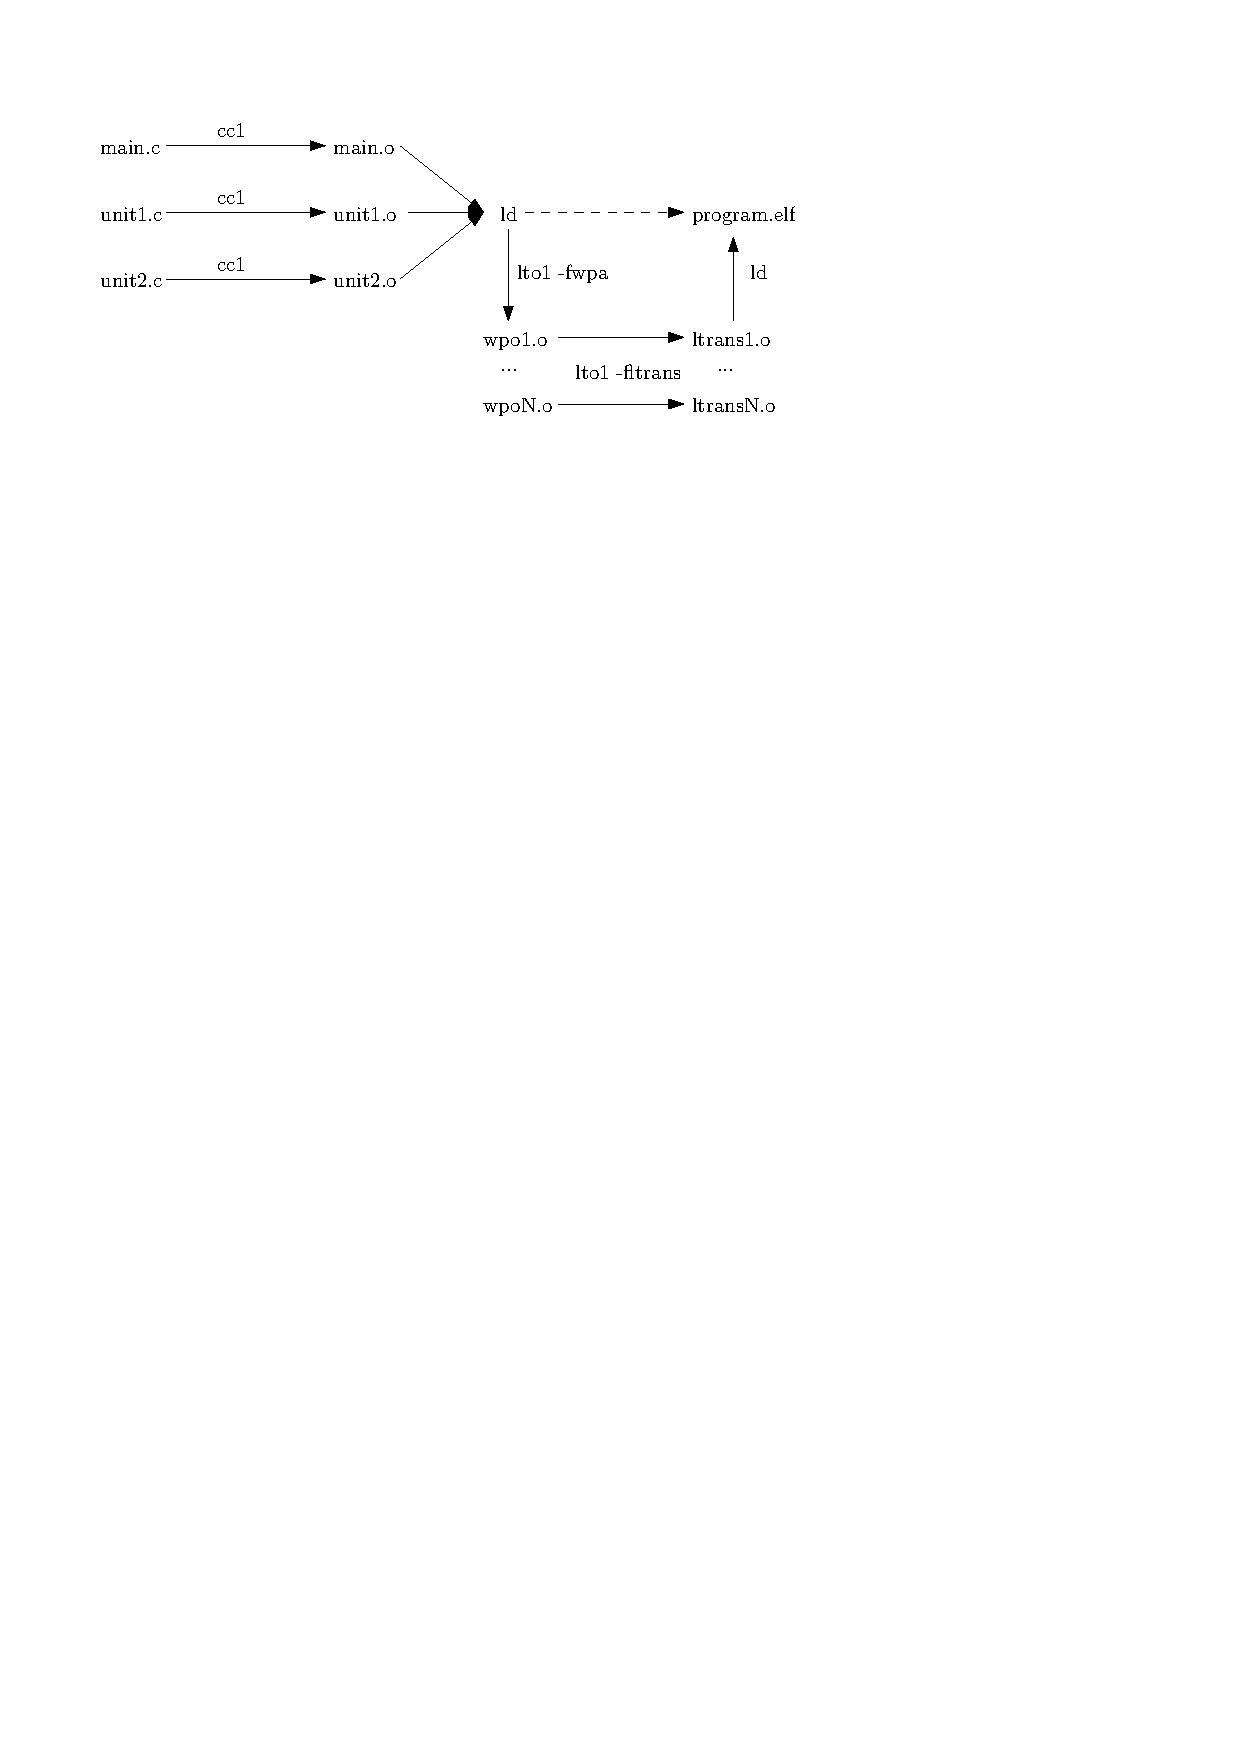
\includegraphics{./img/lto-workflow.pdf}
	\caption{Compiling source code into binary}
	\label{figure-lto-workflow}
\end{figure}

The LTO framework implemented in GCC (see Figure \ref{figure-lto-workflow})
solves these problems by keeping separate compilation, but instead of generating
classical object files containing machine code, the middle end stops and writes
GIMPLE representation into the object, including some metadata (for example the
call graph).

Instead of generating library, the linker then picks up the GIMPLE
representation and invokes the compiler again. GCC was designed to perform most
of the optimizations in parallel, and the process has been further split into
two stages. The sequential WPA (Whole Program Analysis) stage and parallel
LTRANS (Local TRANSformations) stage.

\paragraph{WPA} stage performs declaration and type linking, and decision stage
of interprodecural optimizations. It ends by partitioning the code into smaller
pieces called {\sl LTO partitions}. The partitioning happens with regard to the
code being optimized, for example to minimize cross-partition edges.

\paragraph{LTRANS} stage then performs optimizations decided by WPA stage,
followed by local optimizations and code generation.


\section{Evaluating GCC performance}

As we previously noted, we will be focusing on the GCC suite. In this
section, we will cover the experimental setup, evaluate compile time in selected
programs and extract practical information on resources needed and anticipated
use.  The source code used to take these measurements is available online (See
\TODO{ref}, allowing others to reproduce results presented and use it in future
work.  

\subsection{Compiler}

For further measurements, we the 5.3 release of GCC. This release is relatively
fresh, supports most of the latest features, but formed a stable base for
development and testing. 

\subsection{Tested software packages}

Several opensource programs are available for testing, however a good candidate has
to be selected in order to make testing straightforward and reproducible.
We will choose testing applications based on the following criteria:

\begin{itemize}
	\item written in C++ (preferred) or C,
	\item good compatibility with current GCC versions (5.x and 6.x),
	\item flexible and robust build system,
	\item mid to large codebase,
	\item and preferably large monolithic binary.
\end{itemize}

It is surprisingly difficult to find projects that fit all of those
requirements. For example the build systems of MySQL and Inkscape is very
inflexible and has trouble with LTO compilation. GIMP consists of many plugins
which does not pose any challenge for the current link-time optimizer. The
following applications were used in this work.

\paragraph{Firefox} is already an established benchmark for GCC \cite{glek2010}
and though earlier versiond were difficult to build with LTO, recent versions
are polished and fullfill all the requirements. Is is the largest test case and
though it takes only a few minutes to compile in standard setup, the time can be
raised to many hours with certain optimizations enabled. We will discuss this in
more detail later in Section \ref{section-firefox-lto-pta}. Besides the size,
the codebase is also divers and makes use of modern C++ constructs. The specific
version used in testing is {\it Firefox 48}.

\paragraph{Merkaartor} is an OpenStreetMap editor written in C++ with medium
sized code-base. It utilizes Qt framework, a lot of C++ constructs and links
plenty of objects into a single binary. It also uses a lot of C++ constructs.  The
specific version used in testing is {\it Merkaartor 0.18.3-rc1}

\paragraph{SQLite} is a SQL database engine in a single source file with a
medium (to small) sized code-base. It is the simplest of all three and does not
offer much challenge for the optimizer, but offers very quick turn time as well
as an easy entry point for testcase minimization. The specific version used in
testing is {\it SQLite 3.8.7.4}.

\subsection{Experimental setup}

Where relevant, the following machine was used for testing:

\begin{itemize}
	\item Intel Xeon E3-1231-v3 @ 3.40GHz (Haswell)
	\item 32GB DDR3 RAM @ 1600MHz, 4 modules KHX1600C10D3/8G
	\item 120GB Intel 520 SSD, SSDSC2CW120A3
\end{itemize}

This setup is on the high-end of desktop computing, and much more than
should be required for regular development. 

The system was running 64bit Linux kernel 4.5 and standard Gentoo Linux
installation. Memory and CPU usage measurements were taken using Linux Control
Groups \TODO{cite} for whole compilation process, including GNU make and other tools. The
data were sampled at one second intervals, which is more than enough. Total CPU
usage is known precisely, as control groups keep cumulative counter. The
activity at a given point is used only as a pointer as to how many cores are
currently computing. The measurement is precise enough for memory too, as
we are not allocating and freeing memory rapidly. In fact, most of our
allocations will be done at the beginning of an analysis.

\subsection{Compiling Firefox with LTO and IPA PTA}
\label{section-firefox-lto-pta}

Firefox, in a standard configuration, can be compiled within minutes. See Figure
\ref{figure-firefox-nolto} for a graph of the whole compilation (not only the
{\tt libxul.so}). The dip in CPU cores used around 16th minute is the linker for
{\tt libxul.so} being invoked, the following spike is a parallel compilation of a few
unit tests and miscellaneous parts.

\begin{figure}[h!]
	\centering
	\includegraphics{./graphs/firefox-nolto/firefox-ipa-pta.pdf}
	\caption{Compiling firefox without LTO}
	\label{figure-firefox-nolto}
\end{figure}

Enabling LTO results in slightly longer compile time, but most of the time is
spent during the LTO phase of {\tt libxul.so}, which is plotted separately in Figure
\ref{figure-firefox-lto8}.

Enabling the interprocedural alias analysis pass causes the compilation to end
abruptly due to insufficient RAM.  See Figure \ref{figure-firefox-ipa-pta-lto8}
for details: each drop in utilized CPU cores shows a moment where one LTO
process was killed by the kernel on OOM condition (or finished successfully in
later phases). This issue is remedied by running only 2 processes concurrently
(see Figure \ref{figure-firefox-ipa-pta-lto2}).  However even in this setup the
compiler used more than 27 GB RAM and it took around 18 hours to complete.

\begin{figure}
\begin{subfigure}[b]{\textwidth}
	\centering
	\includegraphics{./graphs/firefox-lto8/firefox-ipa-pta.pdf}
	\caption{{\tt libxul.so} with {\tt -flto=8}}
	\label{figure-firefox-lto8}
\end{subfigure}
\begin{subfigure}[b]{\textwidth}
	\centering
	\includegraphics{./graphs/firefox-ipa-pta-lto8/firefox-ipa-pta.pdf}
	\caption{{\tt libxul.so} with {\tt -fipa-pta -flto=8}}
	\label{figure-firefox-ipa-pta-lto8}
\end{subfigure}
\begin{subfigure}[b]{\textwidth}
	\centering
	\includegraphics{./graphs/firefox-ipa-pta-lto2/firefox-ipa-pta.pdf}
	\caption{{\tt libxul.so} with {\tt -fipa-pta -flto=2}}
	\label{figure-firefox-ipa-pta-lto2}
\end{subfigure}
\caption{Compiling {\tt libxul.so} with different optimization options}
\end{figure}

\subsection{Profiling GCC}

To see what areas of GCC are worth improving, we used {\tt perf} \TODO{cite} to record usage
statistics for various GCC functions. Figure \ref{table-profile-lto} shows top 20 used
functions during LTO phase. It is not surprising to see a lot of {\tt bitmap\_*}
functions, as a lot of passes use bitmaps for computations and storing results.
Typical users are data-flow analyzers \cite{muchnick1997advanced} used many times through the
compilation process, register allocator and points-to analysis. Enabling
interprocedural points-to analysis ({\tt -fipa-pta}) shows drastically different
results, with functions {\tt bitmap\_ior\_into} and {\tt bitmap\_elt\_ior}
taking almost all the CPU time. This clearly shows the pass could benefit from
bitmap and/or algorithm optimizations.

\begin{table}
\centering
\noindent\begin{tabular}{|c|l|l|}\hline Overhead & Cmd/Object & Symbol \\  \hline
\hline$2.92\%$ & \tt ltrans\hfill/lto1 & \tt bitmap\_set\_bit \\
\hline $2.19\%$ & \tt ltrans\hfill/libc & \tt \_int\_malloc \\
\hline $1.92\%$ & \tt ltrans\hfill/lto1 & \tt bitmap\_clear\_bit \\
\hline $1.40\%$ & \tt ltrans\hfill/lto1 & \tt ggc\_internal\_alloc \\
\hline $1.26\%$ & \tt ltrans\hfill/lto1 & \tt record\_reg\_classes \\
\hline $1.16\%$ & \tt ltrans\hfill/lto1 & \tt process\_bb\_lives \\
\hline $1.07\%$ & \tt ltrans\hfill/lto1 & \tt df\_note\_compute \\
\hline $0.91\%$ & \tt ltrans\hfill/lto1 & \tt bitmap\_bit\_p \\
\hline $0.91\%$ & \tt ltrans\hfill/lto1 & \tt df\_ref\_create\_structure \\
\hline $0.88\%$ & \tt wpa\hfill/lto1 & \tt inflate\_fast \\
\hline \end{tabular}

\caption{{\tt perf} profile with {\tt -flto}}
\label{table-profile-lto}
\end{table}

\begin{table}
\centering
\noindent\begin{tabular}{|c|l|l|}\hline Overhead & Cmd/Object & Symbol \\  \hline
\hline $80.99\%$ & \tt ltrans\hfill/lto1 & \tt bitmap\_ior\_into \\
\hline $3.62\%$ & \tt ltrans\hfill/lto1 & \tt bitmap\_set\_bit \\
\hline $2.11\%$ & \tt ltrans\hfill/lto1 & \tt find\_what\_var\_points\_to \\
\hline $1.79\%$ & \tt ltrans\hfill/lto1 & \tt do\_complex\_constraint \\
\hline $0.53\%$ & \tt ltrans\hfill/lto1 & \tt find \\
\hline $0.40\%$ & \tt ltrans\hfill/lto1 & \tt bitmap\_copy \\
\hline $0.38\%$ & \tt ltrans\hfill/lto1 & \tt bitmap\_bit\_p \\
\hline $0.36\%$ & \tt ltrans\hfill/lto1 & \tt bitmap\_elt\_insert\_after \\
\hline $0.35\%$ & \tt ltrans\hfill/lto1 & \tt add\_graph\_edge \\
\hline $0.34\%$ & \tt ltrans\hfill/lto1 & \tt solve\_constraints \\
\hline \end{tabular}

\caption{{\tt perf} profile with {\tt -flto -fipa-pta}}
\label{table-profile-lto-pta}
\end{table}



